\section{Style Transfer}

\noindent Die letzte Technik, auf die wir einen Blick werfen werden, ist der Style Transfer. Diese Technik erlaubt es, den Stil eines Bildes auf ein anderes Bild zu übertragen. Dieser Stil kann dabei sehr unterschiedlich sein, von realistisch bis abstrakt, von Zeichentrick bis Fotografie. Das Prinzip des Style Transfers basiert auf der Trennung von Inhalt und Stil. Der Inhalt eines Bildes ist dabei der eigentliche Bildinhalt, also die Objekte, die auf dem Bild zu sehen sind. Der Stil hingegen ist die Art und Weise, wie das Bild dargestellt wird, also die Farbgebung, die Pinselstriche, die Textur, etc. Das Modell ist schließlich in der Lage den Bildinhalt in eine andere Form zu transformieren. Im Beispiel wurde das Tool ToonMe verwendet, um überzeugende Variationen der ursprünglichen Fotografie zu erzeugen.\\

\begin{figure}[H]
    \centering
    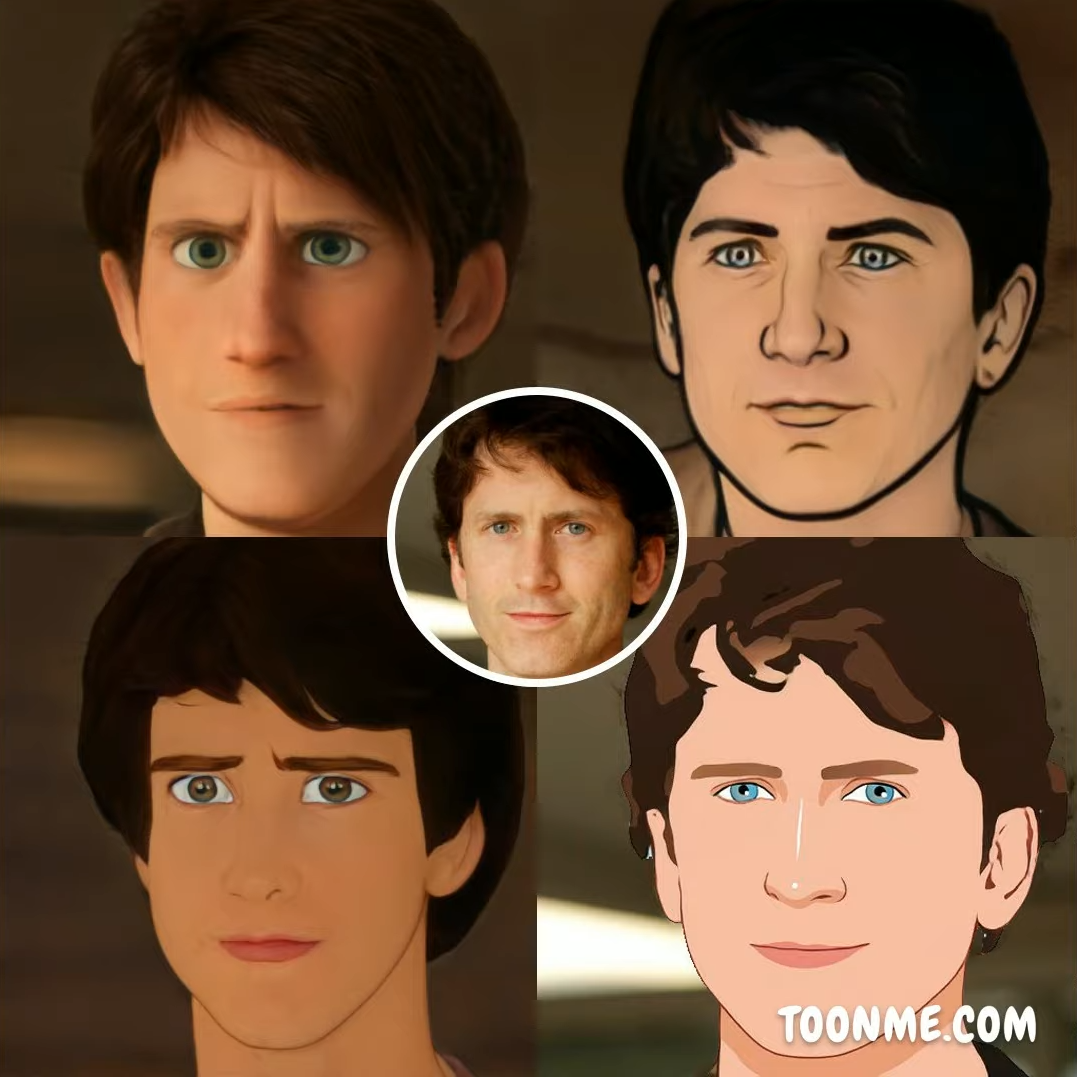
\includegraphics[width=0.8\textwidth]{ToonMe}
    \caption{Style Transfer GAN in der Praxis, Motiv: Todd Howard, Bethesda Softworks} \quelle\url{https://toonme.com} \quelle\url{https://commons.wikimedia.org/}
\label{fig:deep_learning}
\end{figure}

\newpage
